\documentclass{article}
\usepackage{listings}
\usepackage{color}
\usepackage{caption}
\usepackage{graphicx}
\usepackage{oz}
\DeclareGraphicsExtensions{.pdf,.png,.jpg}
\newtheorem{definition}{Definition}
 \usepackage{courier}
 \lstset{
         basicstyle=\footnotesize\ttfamily, % Standardschrift
         %numbers=left,               % Ort der Zeilennummern
         numberstyle=\tiny,          % Stil der Zeilennummern
         %stepnumber=2,               % Abstand zwischen den Zeilennummern
         numbersep=5pt,              % Abstand der Nummern zum Text
         tabsize=2,                  % Groesse von Tabs
         extendedchars=true,         %
         breaklines=true,            % Zeilen werden Umgebrochen
         keywordstyle=\color{red},
    		frame=b,         
 %        keywordstyle=[1]\textbf,    % Stil der Keywords
 %        keywordstyle=[2]\textbf,    %
 %        keywordstyle=[3]\textbf,    %
 %        keywordstyle=[4]\textbf,   \sqrt{\sqrt{}} %
         stringstyle=\color{white}\ttfamily, % Farbe der String
         showspaces=false,           % Leerzeichen anzeigen ?
         showtabs=false,             % Tabs anzeigen ?
         xleftmargin=17pt,
         framexleftmargin=17pt,
         framexrightmargin=5pt,
         framexbottommargin=4pt,
         %backgroundcolor=\color{lightgray},
         showstringspaces=false      % Leerzeichen in Strings anzeigen ?        
 }
 \lstloadlanguages{
         Java
 }
%\DeclareCaptionFont{blue}{\color{blue}} 

 %\captionsetup[lstlisting]{singlelinecheck=false, labelfont={blue}, textfont={blue}}
 % \usepackage{caption}
 
\DeclareCaptionFont{white}{\color{white}}
\DeclareCaptionFormat{listing}{\colorbox[cmyk]{0.43, 0.35, 0.35,0.01}{\parbox{\textwidth}{\hspace{15pt}#1#2#3}}}
 % \captionsetup[lstlisting]{format=listing,labelfont=white,textfont=white, singlelinecheck=false, margin=0pt, font={bf,footnotesize}}



\captionsetup[lstlisting]{format=listing,labelfont=white,textfont=white, singlelinecheck=false, margin=0pt, font={bf,footnotesize}}


\begin{document} 
\bgroup \parindent 0pt
{\Large\textbf{Model Catalogue - version2}}

\vskip 4mm 

{\Large {David Milward}}

\egroup

\vskip 14mm

\noindent

\section{Model Driven Engineering}

\section{Metadata Registry Standards}

In the past Data Dictionaries were used to store details of database record structure or application data structure on a local per application or database basis; a metadata registry provides a similar capability but on a system or organisation-wide basis. It can also provides features that are commonly included in a \emph{thesaurus}, a \emph{Taxonomy}, and an \emph{Ontology} . These features include the ability to classify terms in relation to one another, record relationships such as synonyms, and classify hierarchical relationships. The first large-scale adoption of metadata registries appears to be by the US caBIG initiative~\cite{kunz09} and following on from that there was the  and the caCORE software development kit~\cite{koma08}. Our interest in using Metadata Registry toolkits stems from the work carried out in the CancerGrid project~\cite{davi14}, where an ISO1179-compliant metadata registry was developed for curation of semantic meta data and model-driven generation of trial-specific software~\cite{davi12, Abler2011}. However tests of the XML-based metadata registry indicated that this work require a more scalable solution.



\subsection{ISO11179 The ISO standard for Metadata Registries}

Other approaches have been taken, in~\cite{Sinaci} the authors describe a federated semantic metadata registry framework which based around the ideas of LOD (Linked Open Data) and ISO11179, the main part of the framework being implemented using Jena~\cite{jena}  as an open source project~\cite{semanticmdr} called the Semantic MDR.

Metadata Registries contain the ability to examine both how a data element is represented as well as what it means, and it is this relationship that is embodied in the International Standard 11179(ISO11179) ~\cite{ISO11179}, which we examine in the next section. There are other standards which purport to be concerned with metadata registries namely ISO15000-3 and ISO15000-4, also known as ebXML, however these are more concerned with storing and accessing metadata rather than classifying it and relating the semantic and representational aspects of that metadata for purposes other then simply a metadata repository.

The standard is not formally defined and as a result many of the definitions are scattered over the 6 sections of the ISO11179 documentation, and are quite hard to pull together. The registry itself stores metadata; data which describes, analyses, classifies and manages other data, it needs therefore to be able to document the structure and context of the data being used. The specification of the registry itself is ambiguous and therefore requires further specification for the entities which are being stored. In fact this further documentation is referred to from within the standard to explain the structure and workings of the metadata entities themselves, in particular it references a set of 5 technical reports (up to 134 pages each) also issued by ISO ISO20943~\cite{ISO20943} which examine different aspects of the metadata registry content, in an attempt to standardise the actual metadata being stored to ensure that it is standardised between registries.  


We follow their example in order to try and gain a firm understanding of the concepts within the standard. 

\subsubsection{Data Element Sub-Group}
In this section we will refer to the ISO ISO20943-1 technical report, which is the \emph{data element} chapter of the technical report titled \emph{Procedures for achieving metadata registry(MDR) content consistency}.

In section 1.4 it is pointed out that some \emph{Registration Authorities} choose to register datasets as Value Domains and others register them as data elements, although no guidance is given as to why this should be the case or whether one way is better than the other way. Section 4 of the report then notes that different layers can be built up during the modelling process and that data elements can, according to their structure and relationships, be assigned to different abstraction layers. It notes that data elements can be related using \emph{specialization/generalization, concatenation, and aggregation}, although the report makes no attempt to reference the large body of object oriented software development knowledge which normally provides the context for such terms. Section 4.2 details how a set of different mailing addresses can be formed into hierarchy of addresses by using a combination of data element attributes and Classification Scheme membership. It observes that their may be other areas of the registry where the same elements need to be placed into different hierarchies by using different attributes. 

Section 4.2.1 then continues to identify how if two data elements(Geographic and Mailing Address State Code) are both  descended from the same parent (State USPS Code), and if their respective value domains are the identical then as an alternative representation one can represent this as two data elements sharing the same value domain (which would be called State USPS Code). However there is no guidance as to why one would want to do this, or indeed why one would want the hierarchical representation of data elements. Arguably the main reason for wanting such a hierarchical representation is that it forms part of a \emph{model}, and that \emph{model} uses a hierarchical set of relationships. One may observe that if this is the case then the \emph{model} will probably hold the answer as to whether one or two value domain entities are needed to represented the permissive values required for the data elements.

Section 4.3 details an example of the use of concatenation, or rather shows an organisation diagram of how one might want to organise these entities, however it totally misses the fact that building such a \emph{model} will either done as part of an exercise in \emph{modelling}, \emph{software design} or as a reverse-engineering exercise, perhaps while building up a model from parsing text. In all these exercises there will be a set of rules being followed, and reference to these rules might be a better way of organising the entities.  All this examples does is give one very out of context set of options selected from thousands, and there is very little to be learnt from it apart from the fact that one could possibly concatenate the data elements to full-fill some unstated greater purpose.

Section 4.4 goes on to discuss \emph{aggregation} in the same vague and inconsistent terms, observing that attribute values and data element concepts may need to be changed in order to capture different structures.

Section 5 details the way in which data elements should be registered, and it makes the observation that this can be done from a \emph{top-down} approach, or from a \emph{bottom-up} approach. Interestingly it lists the \emph{bottom-up} approach first, the implication being that whoever is writing the manual expects to be receiving a series of data elements that are not from a previously known and structured data-set. For the purposes of most scientific users people who are integrating existing systems and datasets the top-down approach is probably more useful. 

For the bottom-up approach the report recommends that the \emph{semantic content} of the data element needs to be captured, and refers the reader back to the definitions in the standard in particular in part 4, as well as Annex B, the report then goes on to describe how to handle value domains, again referring to Annex B and also section 3 of the standard. If we look first at part 4 of the standard, firstly we see that part 4 has not been updated in version 3 of the standard, we therefore assume version 2 is the current (normative) reference for this part of the standard. Part 4 is called \emph{Formulation of Data Definitions}, and the first section of this document states that it is dealing with \emph{semantic} definitions rather than formatting (presumably syntactical) definitions. The next two sections specify conformance conditions and give a list of terminological definitions, which are repeated in other parts of the standard, it must be noted that it is rare to see a terminology forming a main section in an international standard, but unfortunately the reasons as to why a terminology forms a main section rather than an annex is not stated. Section 4 then states requirements and recommendations for data definition, we assume it is referring to metadata definition rather than data definition, however this is not stated. What is stated is a list of requirements, such as \emph{A data definition shall state what the concept is, not only what it is not} and recommendations such as \emph{the data definition should state the essential meaning of the concept, it should be precise and unambiguous in among several other recommendations}. It must be observed such considerations been taken seriously by the standard's authors then the standard it might well have been adopted more widely. Section 5 continues in the same vein with 5 examples of \emph{good} and \emph{bad} data definitions, references to other standards, as well as making the observation that the essential meaning of a data element is context dependent. However this observation is not carried through into it's corollary that therefore a metadata registry needs to capture \emph{context} and that this is one of the main features that will make the rest of the definitions redundant. 

Sadly there are no more sections, so we need to inspect Annex B, which is found at the end of part 6 (in this case of version 3 of the standard), it is titled \emph{ Contents of the Metadata Registry: Metadata attributes required for Administered items}. It consists of two tables that detail how each item should be administered, whether it is mandatory, optional , contingent or indicative.  However going back to the ISO ISO20943-1 technical report, section 1.3 (p8), the examples referred to in Annex B don't appear to be there, or if they are they are somehow hidden in the tables in a way which renders them almost completely undecipherable to the untrained eye. 

Continuing with the technical report, section 6.1.5 on page 9 states that it may be appropriate to define and register a \emph{Representational Class}, going on to detail how to register it as an administrative items, rather than detailing how it fits into the overall scheme, or why - since it is optional - one would want to register such an entity. Section 6.1.6 details how to use identifiers and names, which are not defined within the standard although they are used, section 5 of the standard specifies how to document any naming convention used. Section 6.1.7 details other metadata attributes which are required such as origin, comments and other similar ancillary attributes. Section 6.1.8 deals with Data Element Concepts (DEC) and details how these are often related to several data elements, it goes on to explain how a DEC may be identified by using its object class, property and qualifiers. 

In this explanation DEC's are specified through their \emph{Conceptual Domains(CD)} which are defined as a set of value domains. An example is given whereby the CD is given as \emph{Canadian Provinces} with each instance of a province being associated with a specific \emph{Canadian Province Identifier} data element and a specific \emph{value domain} which further specifies the value. This means in a registry one would have a CD containing a value \emph{Canadian Provinces} which would be linked to a DEC called "Canadian Province Identifier", this in turn would \emph{contain} a number od data elements which would be called names such as: Alberta, British Columbia, Manitoba, etc. This explanation states that each province would be represented by a different \emph{value domain}, further stating that each province would be associated with a different \emph{value meaning} which in turn could be represented by a two character code. 

The example itself would be acceptable if it answered the questions that inevitably arise from considering the subject matter, issues such as what exactly is the relationship between a data element and a DEC? Does this relationship or association have other attributes? are they relevant to metadata registry? why not have a \emph{containment} relationship between data elements and the data element concepts? why not use a single value domain with an enumeration to represent the permissive values? 

Unfortunately the \emph{concepts} used in the standard are not governed by any rules, if they were specified in a language such as OWL then we could reason about them, we would be able to see how a particular relationship is registered in the metadata registry. However as things stand the metadata items, the \emph{things} that are being administered inside the MDR are defined in an ambiguous fashion, and thus it is very difficult to reason about them.

The problem with the example given is that the concepts can be mapped to Conceptual Domains, Value Meanings, and Data Element Concept in a seemingly random fashion and no such rules are given on how to adapt this example to other cases in other potentially diverse domains.




\subsubsection{Value Domain Sub-Group}

We examine the third section of the  ISO20943-3 technical report in this next section, the purpose of the technical report is to ensure the equivalent use of metadata between metadata registries which are based on the ISO standard. In section 1.2 the report is defined as being \emph{"a user’s guide for conceptualizing a value domain and its components for the purpose of consistently establishing good quality metadata"}, we learn in 1.3 that the scope is limited to "value domains, conceptual domains, and their associated attributes and relationships" and then in 1.4 that \emph{"There is a choice when registering value domains in an MDR. Some Registration Authorities treat these sets	as value domains, and others treat them as data elements"}.
\begin{quote}
	Value domains are sets of permissible values for data elements.(Definition from part 1 version 3 of the standard - 3.3.38 p9) For example, the data element representing annual household income may have the set of non-negative integers (with units of dollars) as a set of valid values.
\end{quote}
This continues:
\begin{quote}
	A data element concept may be associated with different value domains as needed to form conceptually
	similar data elements. There are many ways to represent similar facts about the world, but the concept for
	which the facts are examples is the same. Take the DEC country of person's birth as an example. ISO 3166
	– Country Codes contains seven different representations for countries of the world. Each one of these seven
	representations contains a set of values that may be used in the value domain associated with the DEC.
	Each one of the seven associations is a data element. For each representation of the data, the permissible
	values, the datatype, the representation class, and possibly the units of measure, are altered.
\end{quote}


ISO/JTC 1/SC 32N2224
2012 (30-4) ISO11179 part 1. 6.1 (p25)
\begin{quote}
	A value domain is a set of permissible values. A permissible value is a combination of some value and the
	meaning for that value. The associated meaning is called the value meaning. A value domain is the set of
	valid values for one or more data elements. It is used for validation of data in information systems and in data
	exchange. It is also an integral part of the metadata needed to describe a data element. In particular, a value
	domain is a guide to the content, form, and structure of the data represented by a data element.
	Value domains come in two (non-exclusive) sub-types:
	⎯ Enumerated value domain – A value domain specified as a list of permissible values (values and their meanings)
	⎯ Non-enumerated value domain – A value domain specified by a description
	An enumerated value domain contains a list of all its values and their associated meanings. Each value and
	meaning pair is called a permissible value. The meaning for each value is called the value meaning.
	A non-enumerated value domain is specified by a description. The non-enumerated value domain
	description describes precisely which permissible values belong and which do not belong to the value
	domain. An example of a description is the phrase "Every real number greater than 0 and less than 1".
\end{quote}
ISO/JTC 1/SC 32N2224
2012 (30-4) ISO11179 part 1. 6.3 (p27)



....tbc


\subsection{Metadata Registry Summary}

It is clear from the previous section that the ISO standard itself has not followed it's own guidelines, it is not clear, it is ambiguous, and it does not stand on its own (for instance it needs at least two further technical reports to ensure metadata compliance). 

The metadata registry is an attempt to marry concepts with metadata, using a flexible adaptable model which can be used for a variety of different use cases. In particular it is intended to capture the meaning of different datasets using metadata, some of structural, some of it relational and some built into the typing of value domains and datatypes.  Currently the standard is lacking in having a way to capture structure and context easily, it measures data elements only in terms of themselves, not in terms of their relationships to other data elements, and it is not really clear whether a metadata registry should have a separate entity called a data element.

We propose two changes to the ISO11179 model in order to solve these problems, firstly we need to introduce the \emph{context} of model driven engineering and allow data elements to be placed within structures that are currently used for grouping data elements in most current information systems. We need to link these structures to the current UML/EMF models available in the Software Engineering world. We need to remove the convoluted systems of conceptual domains and value meanings, and introduce a simpler clearer means of representing the \emph{type} systems which are part of the \emph{Value} aspects of the metamodel. Lastly, we need to devise a framework which will link these structures to the reasoning systems available in the semantic web world.

In the next section we introduce a new design for a metadata registry which we are calling a \emph{Model Catalogue} by:
\begin{itemize}
	\item Introducing Models as a containment for data elements using tried and tested software engineering techniques.
	\itemFormally specifying the \emph{Metamodel} on which the \emph{Model Catalogue} is based.
\end{itemize}

 

 



\section{Architecture}

The model catalogue version 2 is based on the existing model catalogue, but we are building it from scratch using the eclipse EMF model driven stack so that individual aspects of the model can be isolated and for academic reasons studied separately. As new designed elements are proved in the model catalogue 2 stack, we plan to adapt the existing Grails toolkit accordingly, but on an incremental basis.

The main classes in the metamodel are shown, together with their inheritance hierarchy in figure~\ref{fig:inheritance}. These are a \emph{CatalogueCore} class which roughly corresponding with the existing abstract \emph{CatalogueElement} class, it is intended to be an abstract class to which administrative behaviours can be added at a later stage, these will then be available in all the subclasses in the catalogue. We summarise these classes below:
\begin{itemize}
\item Catalogue Core - An abstract class allowing all other classes to be administered, annotated, constrained and associated.
\item DataModel - the main modelling artefact, all other entities will be a part of a DataModel
\item DataConcept - An abstract class which allows all its child classes to be treated as concepts.
\item DataSection - A grouping class for parts of a model, it can contain other DataSections, and DataClasses.
\item DataClass - A container for DataElements.
\item ValueDomain - A structure for the value/ representation of the DataElement composed of Datatypes, MeasurementUnits and Enumerations.
\item Datatype - A class which specifies a particular datatype as a primitive, such as bool or int.
\end{itemize}

 \begin{figure}[here]
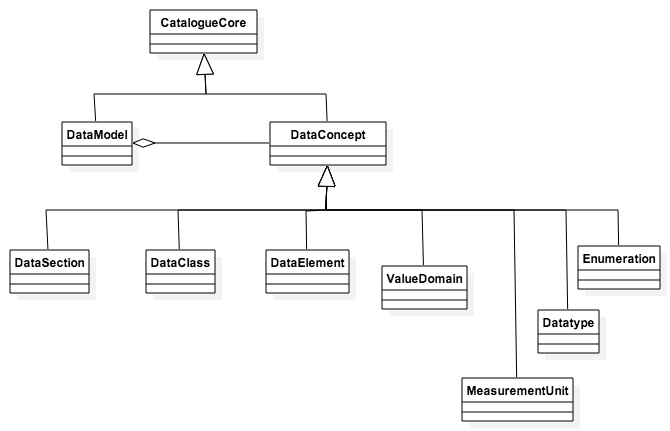
\includegraphics[scale=0.4]{images/inheritance}
\caption{Core Classes - Inheritance Model} 
\label{fig:inheritance}
\end{figure}

Figure~\ref{fig:core1} 



The \emph{CatalogueCore} class is the \emph{parent} of both the \emph{DataModel} and \emph{DataConcept} class, which are shown in figure~\ref{fig:core2} The \emph{DataModel} is a container class for all the models in the model catalogue, is roughly equivalent to the current \emph{Classification};  \emph{DataModels} will be the \emph{entities} that the model catalogue will manage.

 \begin{figure}[here]
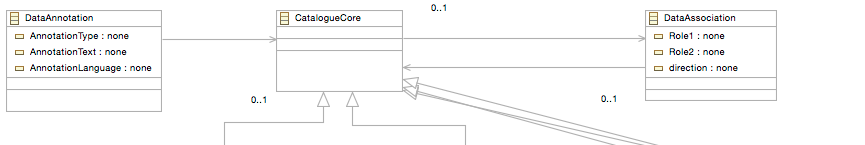
\includegraphics[scale=0.4]{images/core1}
\caption{Core Classes 1} 
\label{fig:core1}
\end{figure}

\subsection{Groupings inside the DataModel}

A \emph{DataAnnotation} class is needed to add annotations to any of the model elements in the model catalogue, and this includes constraints. We are not developing an expressions aspect to the language, at present it is a structural language and hence we adopt the UML practise of including a constraint in an annotation. The annotation will have a type of either text or constraint (not shown yet ) and then it will have the annotation language, which depending on the type will either refer to a spoken language (such as German) or a constraint language (such as OCL).

\begin{figure}[here]
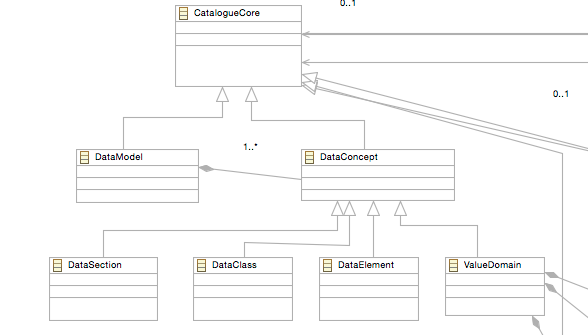
\includegraphics[scale=0.4]{images/core2}
\caption{Core Classes 2} 
\label{fig:core2}
\end{figure}


Since a DataAnnotation is derived from the CatalogueCore entity we are able to write a DataAnnotation about an existing DataAnnotation. We are also able to add a constraint to a class, or a DataAssociation between two separate classes. If we have a DataClass containing a DataElement represented by a ValueDomain with a Datatype of integer, that value domain may itself be constrained in fact in this language we want to maintain constraints at the level of a valuedomain. In stating that a particular blood pressure is a maximum that may be related to a particular context, which means that the maximum may only be applied when there is an association between two data elements, and that association may not be direct.




The class \emph{DataConcept} is an abstract class which is the parent of \emph{DataSection}, \emph{DataClass},\emph{DataElement}, \emph{ValueDomain}. The main idea behind having a single abstract parent class  \emph{DataConcept}  is to capture the notion that \emph{concepts} may be represented by any one of these classes within a model.  

The \emph{DataElement}, \emph{ValueDomain} are directly derived from the ISO11179 metadata registry standard, and correspond closely with the definitions provided within the standard. A data element in the current catalogue \emph{has} a single value domain, this is a one-to-one containment relationship. 

A \emph{DataClass} is simply a container for \emph{DataElements}, it's attributes are limited to \emph{DataElements}, and cannot be  \emph{DataClasses}. There is no upperbound on the number of \emph{DataElements} that can be contained in a \emph{DataClass}. Neither \emph{DataClass} nor \emph{DataElements} have an inheritance mechanism, although they can be associated using the \emph{DataAssociation} mechanism described earlier.

The \emph{DataSection} is a grouping element for \emph{DataElements} and \emph{DataClasses}, it corresponds to section in a documents and is needed as people will always section up large datasets into small digestible \emph{chunks}, normally these will be semantically related and stretch to about 7 entities. It seems sensible therefore to define a separate \emph{grouping} entities to enable this process. 

\subsection{Importing}

Importing can be carried out on any entity which is a child of the CatalogueCore entity, so that while whole DataModels can be imports, so too can DataSections, DataClasses, DataElements and ValueDomains. The standard package notation will apply, so that DataModel will be named using a name and a namespace (normally a URI), and this can be extended using dot notation, so that a DataModel will be identified by \textbf{DataModelName.example.org} and a section could be \textbf{DataSectionName.DataModelName.example.org}, and so forth.

An import will be a reference to an existing finalized DataModel, so that it will not be possible to change any entities within that imported DataModel. If the imported items need to be changed then the \emph{Cloning} operation is required.

\subsection{Cloning}

A clone will act in the same way as an import in terms of specifying the elements to be brought into the new DataModel, however these elements will be copied across as \emph{new and draft} elements into the new DataModel. They can therefore be changed and altered, they may retain an association with the old DataModel, however the association will be a \emph{basedon} type rather than \emph{is}. 



\subsection{Value Domains}

Value domains are entities which define how a \emph{DataElement} is represented in the underlying system, and to do this they can contain \emph{Datatypes}, \emph{Enumerations} and/or \emph{MeasurementUnits}. 

In the simplest example a \emph{DataElement} - say speed, can be represented by a \emph{ValueDomain} which has an integer \emph{Datatypes}. A  \emph{ValueDomain} entity being descended from a \emph{CatalogueCore} can then have a Constraint type of \emph{DataAnnotation} added which limits the speed to a value relative to the system under question, for boats perhaps a speed with an upper limit constraint of 600 (511 being the current world water speed record), and \emph{MeasurementUnits} of kph. 

The idea of a separate entity for measurement units is not completely neccessary as we could put that information into a \emph{DataAnnotation}.


\begin{figure}[here]
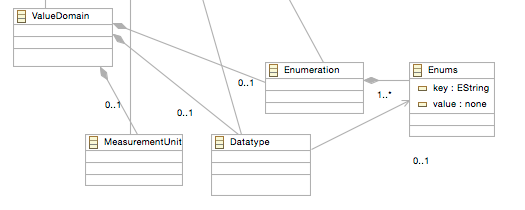
\includegraphics[scale=0.4]{images/core3}
\caption{Core Classes 3} 
\label{fig:core3}
\end{figure}



\newpage

\bibliographystyle{plain}

\bibliography{references}

\end{document}